\documentclass[9pt]{beamer}
\usefonttheme{professionalfonts}
\usetheme[subsectionpage=progressbar]{metropolis}
\setbeamertemplate{section in toc}[sections numbered]
\setbeamertemplate{subsection in toc}[subsections numbered]

\title{The Performance of \\ Physics Informed Neural Networks on \\ Metric Graphs}
\author{Tom-Christian Riemer}
\institute{TU Chemnitz}
\date{March 18th 2022}

%packages
\usepackage{amsmath}
\usepackage[british]{babel}
\usepackage[utf8]{inputenc}
\usepackage{enumerate}
\usepackage{graphicx}
\usepackage{mathtools}
\usepackage{color}
\usepackage{listings}
\usepackage{algpseudocode}
\usepackage{algorithm}
\usepackage{numapde-manifolds}
\usepackage{xcolor}
\usepackage{comment}
\usepackage{varwidth}
\usepackage{subcaption}
\usepackage{blkarray}

\lstset{basicstyle=\ttfamily,	tabsize=2}

\newcommand\myeq{\stackrel{\mathclap{\mbox{$def$}}}{=}}

\newcommand{\Pb}[1]{\expandafter\hat#1}

\begin{document}

\maketitle

\begin{frame}{Contents}
  \tableofcontents
\end{frame}

\section{Introduction}

\begin{frame}{Graphs}
  \begin{minipage}{0.5\textwidth}
      \begin{itemize}
          \item $\Gamma = \left(\mathcal{V}, \mathcal{E} \right),$ \\ $\mathcal{V} = \left\{ v_i \right\}_{i = 1, \ldots, V}, \; V = \abs{\mathcal{V}} \in \mathbb{N},$ \\
          $\mathcal{E} = \left\{ e_i \right\}_{i = 1, \ldots, E}, \; E = \abs{\mathcal{E}} \in \mathbb{N}$.
          \item $\forall e \in \mathcal{E} \colon \; e = \left( v^{\operatorname{o}}, v^{\operatorname{t}} \right)$, \\
            $v^{\operatorname{o}}, v^{\operatorname{t}} \in \mathcal{V}$.
          \item Adjacency: $v_1, v_2 \in \mathcal{V}$ \\ $v_1 \sim v_2 \Leftrightarrow \exists e \in \mathcal{E}$ s.t. $v_2$ can be reached from $v_1$ via this edge $e$. \\
          \begin{equation*}
            A^{\Gamma} = 
            \begin{blockarray}{ccccc}
                v_1 & v_2 & v_3 & v_4 \\
                \begin{block}{(cccc)c}
                    0 & 1 & 0 & 0 & v_1 \\
                    0 & 0 & 0 & 1 & v_2 \\
                    0 & 1 & 0 & 1 & v_3 \\
                    0 & 1 & 0 & 0 & v_4 \\
                \end{block}
            \end{blockarray}
        \end{equation*}
      \end{itemize}
  \end{minipage} \hfill
  \begin{minipage}{0.45\textwidth}
      \begin{figure}[H]
          \resizebox{40mm}{40mm}
          {
              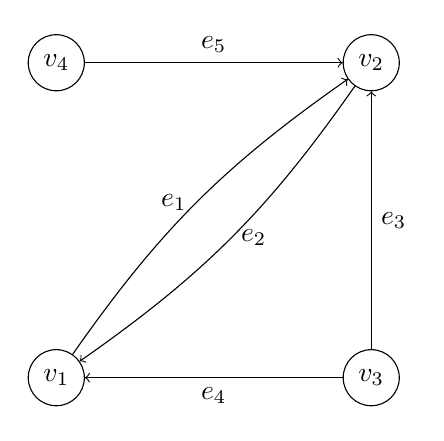
\begin{tikzpicture}
                  % vertices
                  \node[shape=circle,draw=black] (v4) at (0,4) {$v_4$};
                  \node[shape=circle,draw=black] (v2) at (4,4) {$v_2$};
                  \node[shape=circle,draw=black] (v1) at (0,0) {$v_1$};
                  \node[shape=circle,draw=black] (v3) at (4,0) {$v_3$};
                  
                  % edges
                  \path [->](v3) edge node[below] {$e_4$} (v1);
                  \path [->](v2) edge [bend left = 10] node[right]{$e_2$} (v1);
                  \path [->](v1) edge [bend left = 10] node[left]{$e_1$} (v2);
                  \path [->](v3) edge node[right] {$e_3$} (v2);
                  \path [->](v4) edge node[above] {$e_5$} (v2);
              \end{tikzpicture}
          }
      \end{figure}
  \end{minipage}
\end{frame}

\begin{frame}{Metric Graphs}
    \vspace{-1\baselineskip}\hfill{\tiny{[Berkolaiko, Kuchment, 2013]}} \\
    \begin{minipage}{0.5\textwidth}
        \begin{itemize}
            \item Reversal: $e_1, e_2 \in \mathcal{E} \colon e_1 = \overline{e_2}$ \\
            $\Leftrightarrow e_1 = \left( v_1, v_2 \right), e_2 = \left( v_2, v_1 \right)$.
        \end{itemize} 
        \noindent \\
        \textbf{Metric Graph}
        \begin{itemize}
            \item $\forall e \in \mathcal{E} \colon \, \exists \ell_e > 0$.
            \item $\ell_{e_1} = \ell_{\overline{e_1}} = \ell_{e_2} = \ell_{\tilde{e}}$.
            \item $x_{e_1} \in [0, \ell_{e_1}] \colon \, x_{e_1} = \ell_{e_2} - x_{e_2}$.
            \item $\operatorname{dist}(v_i, v_j) = \sum^{N}_{k = 1} \ell_{e_k}$, \\ where $\left\{ e_k \right\}_{k = 1, \ldots, N}$ is path of minimal length.
        \end{itemize}
    \end{minipage} \hfill
    \begin{minipage}{0.45\textwidth}
        \begin{figure}[H]
            \includegraphics[scale=0.15]{img/diagram-20220315 (2).png}
        \end{figure}
    \end{minipage}
\end{frame}
  

\begin{frame}{Metric Graphs}
    $L_2(e)$:
    \begin{equation*}
        \lVert f \rVert^{2}_{L_2(e)} \coloneqq \int_e \lvert f(x) \rvert^2 \, \textup{d} x < \infty.
    \end{equation*}
    $L_2(\Gamma) = \bigotimes_{e \in \mathcal{E}} L_2(e)$:
    \begin{equation*}
        \lVert f \rVert^{2}_{L_2(\Gamma)} \coloneqq \sum_{e \in \mathcal{E}} \lVert f \rVert^{2}_{L_2(e)} < \infty.
    \end{equation*}
    $H^1 (e)$:
    \begin{equation*}
        \lVert f \rVert^{2}_{H^1(e)} \coloneqq \int_e \lvert f(x) \rvert^2 + \lvert f^{\prime}(x) \rvert^2 \, dx < \infty.
    \end{equation*}
    $H^1 (\Gamma) =  \bigotimes_{e \in \mathcal{E}} H^1 (e) \cap C^{0}(\Gamma)$:
    \begin{equation*}
        \lVert f \rVert^{2}_{H^1 (\Gamma)} \coloneqq \sum_{e \in \mathcal{E}} \lVert f \rVert^{2}_{H^1 (e)} < \infty.
    \end{equation*}
\end{frame}

\end{document}
